%------------------------------------------------------------


\begin{frame}
\frametitle{The U Rune}
\begin{columns}[c] % The "c" option specifies centered vertical alignment while the "t" option is used for top vertical alignment

\column{.2\textwidth} % Left column and width
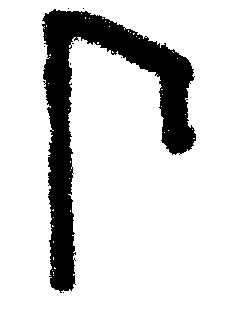
\includegraphics[width=\linewidth]{RuneU.png}
\column{.4\textwidth} % Right column and width
\textbf{\textit{Germanic} Meaning}\\
The \structure{letter U}. \\
\structure{\textit{Uruz}, the aurochs}
\\
Bull, bound energy, earth and primordial energy, drives, health

\column{.4\textwidth} % Right column and width
\textbf{Spiritual Meaning}\\
\structure{passive -- earth force}\\

Rooting, fiery (life) energy, creates the base for forceful actions.
\end{columns}

\vspace{5mm}
\textbf{\structure{U}: The rune of the \structure{healer}}\\
The healer is strongly \structure{rooted and connected to the earth} in order to be able to stay in equilibrium. The exercise let's us take up the needed energy and give off excess energy, so that the energy in the body  can flow unhindered. 
The exercise can be performed in a \structure{squatting position}. Thee rooting might be experienced different.
\end{frame}
%------------------------------------------------------------
%------------------------------------------------------------
\begin{frame}
\frametitle{The I Rune}
\begin{columns}[c] % The "c" option specifies centered vertical alignment while the "t" option is used for top vertical alignment

\column{.2\textwidth} % Left column and width
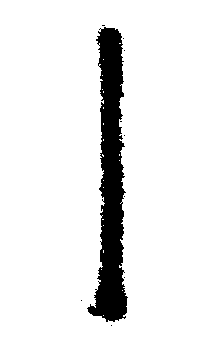
\includegraphics[width=\linewidth]{RuneI.png}
\column{.4\textwidth} % Right column and width
\textbf{\textit{Germanic} Meaning}\\
The \structure{letter I}. \\
\structure{\textit{Isa}, ice, primordial matter.}
\\
Ice, congealment, the I, being yourself, patience, helps to focus on the essential.

\column{.4\textwidth} % Right column and width
\textbf{Spiritual Meaning}\\
\structure{active -- clarity}\\

the clarity of the mind, but also the risk of the congealment.
\end{columns}

\vspace{5mm}
\textbf{\structure{I}: The \structure{ice} rune, ancient matter}\\
According to old germanic legends, the \structure{universe got created from fire and ice}. In the cold, represented by ice, the metabolism and energy levels of our life mellow, whereby intent unfolds only slowly and patience becomes a bitter necessity.
\end{frame}
%------------------------------------------------------------
%------------------------------------------------------------


\begin{frame}
\frametitle{The Y Rune}
\begin{columns}[c] % The "c" option specifies centered vertical alignment while the "t" option is used for top vertical alignment

\column{.28\textwidth} % Left column and width
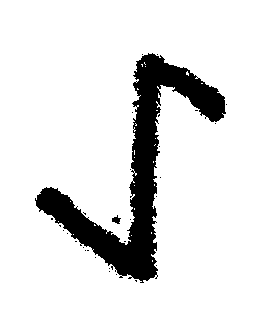
\includegraphics[width=\linewidth]{RuneY.png}
\column{.4\textwidth} % Right column and width
\textbf{\textit{Germanic} Meaning}\\
The \structure{letter Y}. \\
\structure{\textit{Ingwaz (Yngvi)}, God of Ing.}
\\
Peace, calm, serenity, fertility, ripening, egg

\column{.4\textwidth} % Right column and width
\textbf{Spiritual Meaning}\\
\structure{passive -- egg}\\

Set your goal, let your plans ripen in a sheltered place.
\end{columns}

\vspace{5mm}
\textbf{\structure{Y}: The rune of \structure{fertility}}\\
\structure{The egg} which needs to be incubated in a sheltered place. Each idea needs a basis thought, each plant \structure{a seed, a ripening process and care} till the moment of the realisation or harvest.
\end{frame}
%------------------------------------------------------------
%------------------------------------------------------------

\begin{frame}
\frametitle{The F Rune}
\begin{columns}[c] % The "c" option specifies centered vertical alignment while the "t" option is used for top vertical alignment

\column{.28\textwidth} % Left column and width
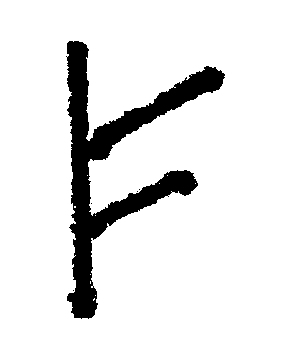
\includegraphics[width=\linewidth]{RuneF.png}
\column{.4\textwidth} % Right column and width
\textbf{\textit{Germanic} Meaning}\\
The \structure{letter F}. \\
\structure{\textit{Fehu}, cattle}
\\
cattle herd, mobile assets, richness, fertility, chaos, energy, fire, money, gold

\column{.4\textwidth} % Right column and width
\textbf{Spiritual Meaning}\\
\structure{active -- the horns of the cattle herd}\\

The \structure{basic of each beginning}.
\end{columns}

\vspace{5mm}
\textbf{\structure{F}: The rune of \structure{love, peace, abundance and fertility}.}\\
This rune \structure{provides} everything there is with energy, no matter if \structure{spiritual, emotional or tangible energy}. \\
Too much energy can be equilibrated with the U rune.
\end{frame}
%------------------------------------------------------------
%------------------------------------------------------------

\begin{frame}
\frametitle{The T Rune}
\begin{columns}[c] % The "c" option specifies centered vertical alignment while the "t" option is used for top vertical alignment

\column{.29\textwidth} % Left column and width
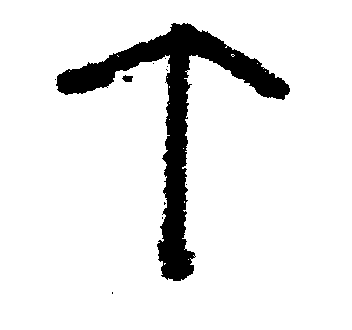
\includegraphics[width=\linewidth]{RuneT.png}
\column{.4\textwidth} % Right column and width
\textbf{\textit{Germanic} Meaning}\\
The \structure{letter T}. \\
\structure{\textit{Tiwaz}, God of Tyr.}
\\
Justice, combat, dignity, drive, determined, motivated.

\column{.4\textwidth} % Right column and width
\textbf{Spiritual Meaning}\\
\structure{active -- \structure{spear of arrow}}\\

The \structure{driven, bring an idea to unfold, to become reality}.
\end{columns}

\vspace{5mm}
\textbf{\structure{T}: The rune of the \structure{divine, invincible warrior}, as well a symbol of a \structure{ruthless drive}.}\\
An idea which gets hold for too long can reach it's goal. Develop a strategy to achieve your goal. Plan your endeavour, visualize your goals, realistically asses the obstacles and  dangers. To reach the the goal where' a will is easier.
\end{frame}
%------------------------------------------------------------
%------------------------------------------------------------

\begin{frame}
\frametitle{The W Rune}
\begin{columns}[c] % The "c" option specifies centered vertical alignment while the "t" option is used for top vertical alignment

\column{.2\textwidth} % Left column and width

\includegraphics[width=\linewidth]{RuneW.png}
\column{.4\textwidth} % Right column and width
\textbf{\textit{Germanic} Meaning}\\
The \structure{letter W}. \\
\structure{\textit{Wunjo}, blissfulness.}
\\
Happiness, joy, finding the measure and equilibrium in life, solidifying the joy of life.

\column{.4\textwidth} % Right column and width
\textbf{Spiritual Meaning}\\
\structure{passive -- \structure{tribal flag}}\\

The \structure{blissfulness and amity}.
\end{columns}

\vspace{5mm}
\textbf{\structure{W}: The rune of \structure{joy, luck, the right measure and equilibrium in life}.}\\
This rune is able too equilibrate different forces. The one who found the path of his soul will effortlessly meet other people whoo are interested in the same things. A community without hierarchy.
\end{frame}
